\chapter{Solaio}
In questo capitolo si affronterà il progetto e la verifica del travetto componente il solaio.
Il travetto si ricorda ha una altezza utile $d=\SI{200}{\milli\metre}$, una base maggiore $B=\SI{500}{\milli\metre}$ e una minore $b=\SI{120}{\milli\metre}$

\section{Progetto preliminare azione flettente}
Il metodo di verifica è pressoché il medesimo di quanto visto nel capitolo relativo al progetto della trave, la grande differenza sta nel fatto che la base non è costante e che occorre controllare dove cada l'asse neutro: se non taglia l'anima, occorre riprogettare il solaio.

Il maggior momento flettente di campata lo si ha nella terza ed è pari a \SI{10.80}{\kilo\newton\metre}, mentre il massimo in appoggio è pari \SI{-15.57}{\kilo\newton\metre}.

\begin{equation}
    \begin{cases}
      b \, \psi \, \xi \, d \, f_{cd} - A_s \, f_{yd} = 0 \\
      A_s \, f_{yd} \left(d - \lambda\,x\right) = M_{Ed}
    \end{cases}
  \end{equation}

Riportando il sistema risolvente simile a quello precedente di pagina \pageref{eq:sistemaSLU}, nel quale $A_s^\prime$ ora non viene considerato, è possibile adottare un minimo di armatura pari a 2Ø14. 
Sapendo di avere problemi per taglio negli appoggi si tende ad adottare 3Ø14 fin da subito agli appoggi sia superiormente che inferiormente, e 2Ø14 nelle campate, solo nella parte tesa. 
L'obiettivo è di cercare di non esser costretti poi a togliere una fila di pignatte o a usare un doppio travetto.

\section{Momento aggiuntivo agli appoggi}
Essendo la struttura agli estremi non realmente con vincoli ad appoggio, la normativa impone di considerarli come degli incastri con un fattore dimezzato a quanto si avrebbe nella campata adiacente, ovvero:
\[
    M_{Ed}^{A1} = \frac{Q_\textup{Camp1} \, l_1^2 }{16} =  \SI{6.022}{\kilo\newton\metre} \quad M_{Ed}^{A4} = \frac{Q_\textup{Camp3} \, l_3^2 }{16} =  \SI{7.795}{\kilo\newton\metre} \quad ,
\]
pertanto agli appoggi di estremità andrà necessariamente una armatura resistente a momento.

\section{Verifica momento flettente}
Con le considerazioni fatte sopra la verifica a momento flettente è largamente soddisfatta. 
In tabella \ref{tab:ULS_M_solaio_VerificaSezioni} sono riportati i dati riassuntivi.
Le ipotesi fatte sono inoltre rispettate.

\begin{table}[htb]
    \centering
    \scriptsize
    \caption[Riassunto della verifica SLU a momento flettente per tutte le sezioni]{Riassunto della verifica SLU a momento flettente per tutte le sezioni}
    \label{tab:ULS_M_solaio_VerificaSezioni}
    \begin{tabular}{
        l
        c
        c
        c
        S[table-format=3.3]
        l
        S[table-format=2.2]
        S[table-format=2.2]
        S[table-format=2.2]
        S[table-format=1.4]
        S[table-format=1.4]
        S[table-format=1.4]
        S[table-format=3.3]
        r
        S[table-format=2.1]}
    \toprule
    \multirow{2}{*}{Sez.}   & {$b$} & \multirow{2}{*}{$A_s$}    & \multirow{2}{*}{$A_s^\prime$} & {$M_{Ed}$}                    & \multirow{2}{*}{Campo}    & {$\varepsilon_c$}         & {$\varepsilon_s$}         & {$\varepsilon_s^\prime$}  & \multicolumn{1}{c}{\multirow{2}{*}{$\xi$}}    & \multicolumn{1}{c}{\multirow{2}{*}{$\psi$}}   & \multicolumn{1}{c}{\multirow{2}{*}{$\lambda$}}    & {$M_{Rd}$}                    & \multicolumn{2}{l}{$M_{Ed}<M_{Rd}$} \\
                            &     {\si{[\milli\metre]}}   &                    &                               & {\si{[\kilo\newton\metre]}}   &                           &{\si{[\textperthousand]}}  &{\si{[\textperthousand]}}  &  {\si{[\textperthousand]}} &                        &                           &                               & {\si{[\kilo\newton\metre]}}   & & {\si{[\percent]}}\\
    \midrule
    A1 inv & 500 & 2Ø14 & 2Ø14 & 6.020  & 2A-1 & 1.93 & 10.00 & -0.46 & 0.1617 & 0.6545 & 0.3728 & 32.907 & \checked & 18.3 \\
    C1     & 120 & 2Ø14 & 0Ø14 & 8.310  & 3B   & 3.50 & 4.50  & 1.90  & 0.4377 & 0.8095 & 0.4160 & 19.707 & \checked & 42.2 \\
    A2 inv & 500 & 3Ø14 & 3Ø14 & 15.670 & 2A-2 & 2.35 & 10.00 & -0.12 & 0.1900 & 0.7158 & 0.3861 & 37.623 & \checked & 41.6 \\
    C2     & 120 & 2Ø14 & 0Ø14 & 11.730 & 3B   & 3.50 & 4.50  & 1.90  & 0.4377 & 0.8095 & 0.4160 & 19.707 & \checked & 59.5 \\
    A3 inv & 500 & 3Ø14 & 3Ø14 & 17.450 & 2A-2 & 2.35 & 10.00 & -0.12 & 0.1900 & 0.7158 & 0.3861 & 37.623 & \checked & 46.4 \\
    C3     & 120 & 2Ø14 & 0Ø14 & 10.720 & 3B   & 3.50 & 4.50  & 1.90  & 0.4377 & 0.8095 & 0.4160 & 19.707 & \checked & 54.4 \\
    A4 inv & 500 & 3Ø14 & 3Ø14 & 7.795  & 2A-2 & 2.35 & 10.00 & -0.12 & 0.1900 & 0.7158 & 0.3861 & 37.623 & \checked & 20.7 \\
    \midrule
    A1     & 500 & 2Ø14 & 2Ø14 & 6.020  & 2A-1 & 1.93 & 10.00 & -0.46 & 0.1617 & 0.6545 & 0.3728 & 32.907 & \checked & 18.3 \\
    C1 inv & 120 & 0Ø14 & 2Ø14 & 1.280  & 2A-1 & 1.85 & 10.00 & -0.52 & 0.1558 & 0.6389 & 0.3704 & 11.795 & \checked & 10.9 \\
    A2     & 500 & 3Ø14 & 3Ø14 & 0.000  & 2A-2 & 2.35 & 10.00 & -0.12 & 0.1900 & 0.7158 & 0.3861 & 37.623 & \checked & 0.0 \\
    C2 inv & 120 & 0Ø14 & 2Ø14 & 0.000  & 2A-1 & 1.85 & 10.00 & -0.52 & 0.1558 & 0.6389 & 0.3704 & 11.795 & \checked & 0.0 \\
    A3     & 500 & 3Ø14 & 3Ø14 & 0.000  & 2A-2 & 2.35 & 10.00 & -0.12 & 0.1900 & 0.7158 & 0.3861 & 37.623 & \checked & 0.0 \\
    C3 inv & 120 & 0Ø14 & 2Ø14 & 0.000  & 2A-1 & 1.85 & 10.00 & -0.52 & 0.1558 & 0.6389 & 0.3704 & 11.795 & \checked & 0.0 \\
    A4     & 500 & 3Ø14 & 3Ø14 & 7.795  & 2A-2 & 2.35 & 10.00 & -0.12 & 0.1900 & 0.7158 & 0.3861 & 37.623 & \checked & 20.7 \\
    \bottomrule
    \end{tabular}
    \end{table}

\section{Verifica a taglio}
La verifica è taglio è affidata solo al contributo lato calcestruzzo senza possibilità di armatura specifica: per questo è più gravosa.
Inoltre in tutte le sezioni occorre considerare la base minore, sia invertite che non. 
La formula di verifica è la medesima di quella riportata a pagina \pageref{eq:Taglio_only_cls}:
\begin{equation}
    V_{Rd} = \max \left\{ \left(\frac{0.18 \, k \, (100 \, \rho_l \, f_{ck})^{\tfrac{1}{3}}}{\gamma_c} + 0.15 \, \sigma _{cp}\right) b_w d \; ; \;(\nu_{min} + 0.15\sigma _{cp}) \, b_w \, d \right\} \quad .
\end{equation}
I risultati sono riportati in tabella \ref{tab:V_no_specific_armor_solaio}.
\begin{table}[htb]
    \centering
    \scriptsize
    \caption{Riassunto della verifica a taglio SLU con resistenza affidata solo al calcestruzzo e senza armatura}
    \label{tab:V_no_specific_armor_solaio}
    \begin{tabular}{
        l
        c
        S[table-format=3.3]
        S[table-format=1.2]
        S[table-format=1.2]
        S[table-format=1.2]
        S[table-format=1.2]
        S[table-format=3.3]
        S[table-format=3.3]
        S[table-format=3.3]
        c
        S[table-format=2.1]}
    \toprule
    \multirow{2}{*}{Sez.} & \multirow{2}{*}{$A_{sl}$} & {$V_{Ed}$} & {\multirow{2}{*}{$k$}} & {\multirow{2}{*}{$\nu_{min}$}} & {$\rho_l$} & {$\sigma_{cp}$} & {$V_{Rd,1}$} & {$V_{Rd,2}$} & {$V_{Rd}$} &  \multicolumn{2}{l}{$V_{Ed}<V_{Rd}$} \\
     & &{\si{[\kilo\newton]}} & & &{\si{[\percent]}}&{\si{[\mega\pascal]}}&{\si{[\kilo\newton]}}&{\si{[\kilo\newton]}}&{\si{[\kilo\newton]}}& &{\si{[\percent]}}\\
    \midrule
    A1 dx & 2Ø14 & 11.420 & 2.00 & 0.49 & 0.01 & 0.00 & 18.300 & 0.000 & 18.300 & \checked & 62.4 \\
    A2 sx & 3Ø14 & 18.240 & 2.00 & 0.49 & 0.02 & 0.00 & 20.948 & 0.000 & 20.948 & \checked & 87.1 \\
    A2 dx & 3Ø14 & 20.170 & 2.00 & 0.49 & 0.02 & 0.00 & 20.948 & 0.000 & 20.948 & \checked & 96.3 \\
    A3 sx & 3Ø14 & 20.820 & 2.00 & 0.49 & 0.02 & 0.00 & 20.948 & 0.000 & 20.948 & \checked & 99.4 \\
    A3 dx & 3Ø14 & 19.950 & 2.00 & 0.49 & 0.02 & 0.00 & 20.948 & 0.000 & 20.948 & \checked & 95.2 \\
    A4 sx & 3Ø14 & 12.910 & 2.00 & 0.49 & 0.02 & 0.00 & 20.948 & 0.000 & 20.948 & \checked & 61.6 \\
    
    \bottomrule
    \end{tabular}
    \end{table}

\section{Lunghezza ancoraggio e traslazione diagramma}
\paragraph{Lunghezza ancoraggio}
Il procedimento di calcolo della lunghezza di ancoraggio è identico a quanto già visto per la trave, considerando i coefficienti $alpha$ e $\eta$ i medesimi, quello che varia è il diametro delle barre:
\begin{equation}
l_{b} = l_{b,req} 
= d_{barre} \frac{ \sigma_{d} }{ 4 \cdot f_{bd} }  
= \SI{14}{\milli\metre}  \frac{ \SI{391.304}{\mega\pascal} }{ 4 \cdot \SI{2.693}{\mega\pascal} } 
= \SI{508.517}{\milli\metre}  
\end{equation}

\paragraph{Traslazione diagramma}
Analogamento a quanto fatto per la trave, ciò che governa l'equazione è l'altezza utile $d$, per cui:
\begin{equation}
    a_1 = \frac{0.9 \, \SI{200}{\milli\metre} \, 2.5}{2} = \SI{0.225}{\metre} \quad .
\end{equation}

In figura \ref{fig:ULS_M_ULS_M_DisposioneArmature_solaio} e \ref{fig:ULS_M_ULS_V_DisposioneArmature_solaio} sono riportate la sovrapposizione di azioni agenti e azioni resistenti, con indicazione inoltre della lunghezza di ancoraggio.

\begin{figure}[htb]
    \centering
    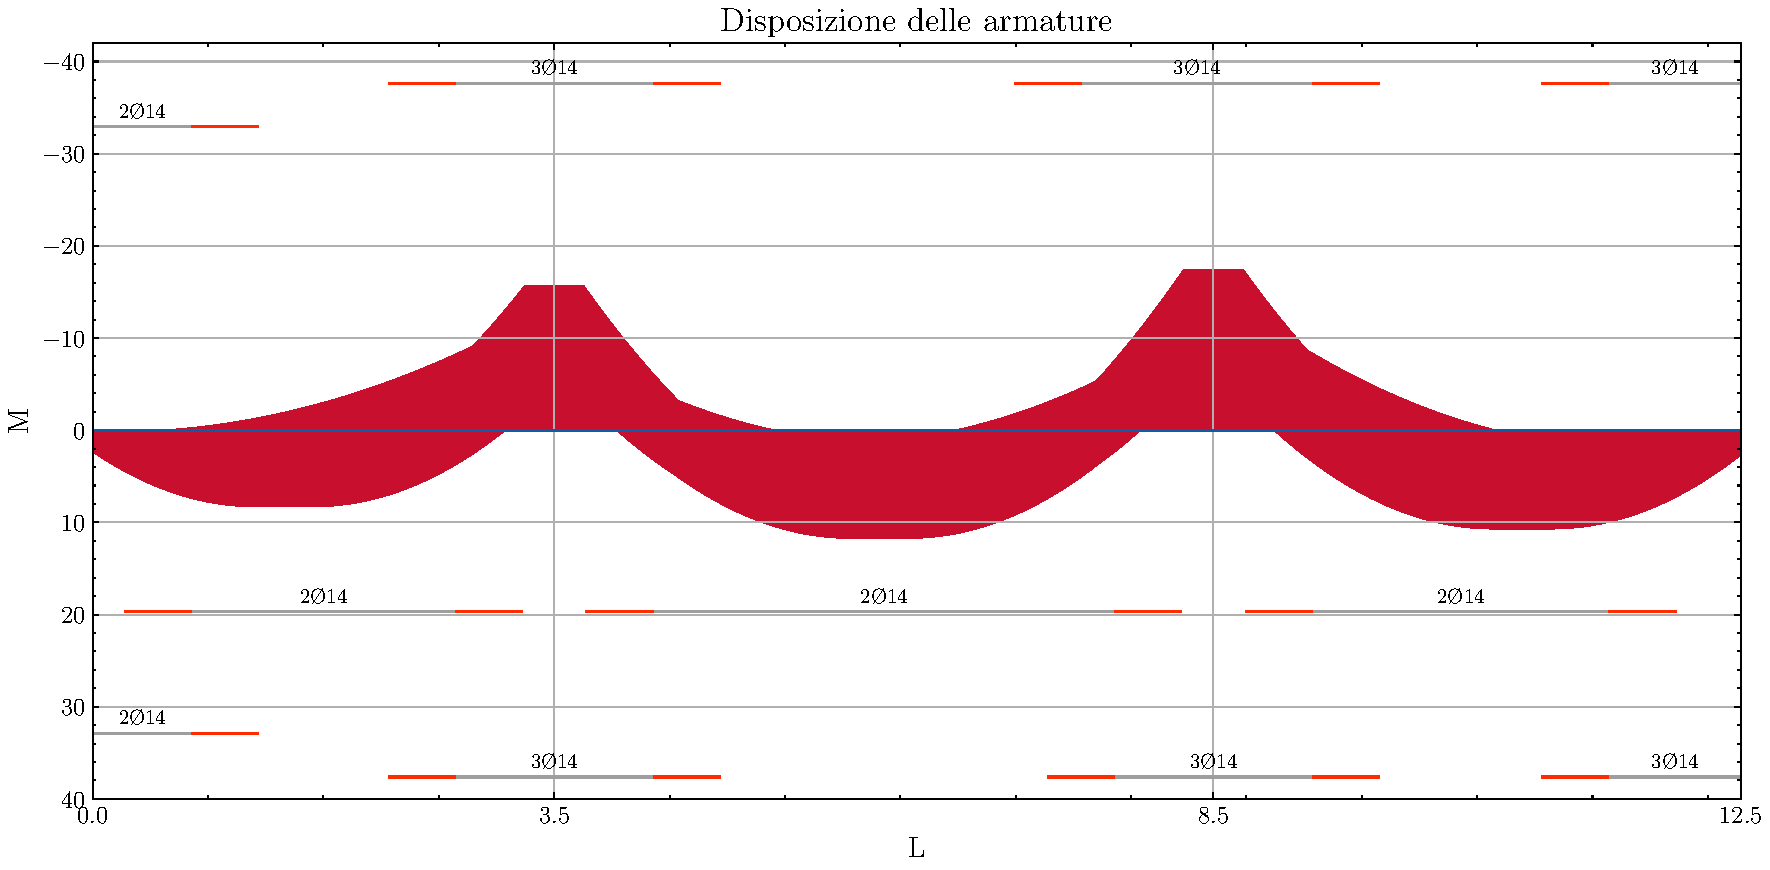
\includegraphics[width=\textwidth]{IMG/ULS_M_DisposioneArmature_solaio.pdf}
    \caption{Disposizione schematica della armatura con raffigurazione della lunghezza di ancoraggio e sovrapposizione momento resistente con momento agente}
    \label{fig:ULS_M_ULS_M_DisposioneArmature_solaio}
\end{figure}
\begin{figure}[htb]
    \centering
    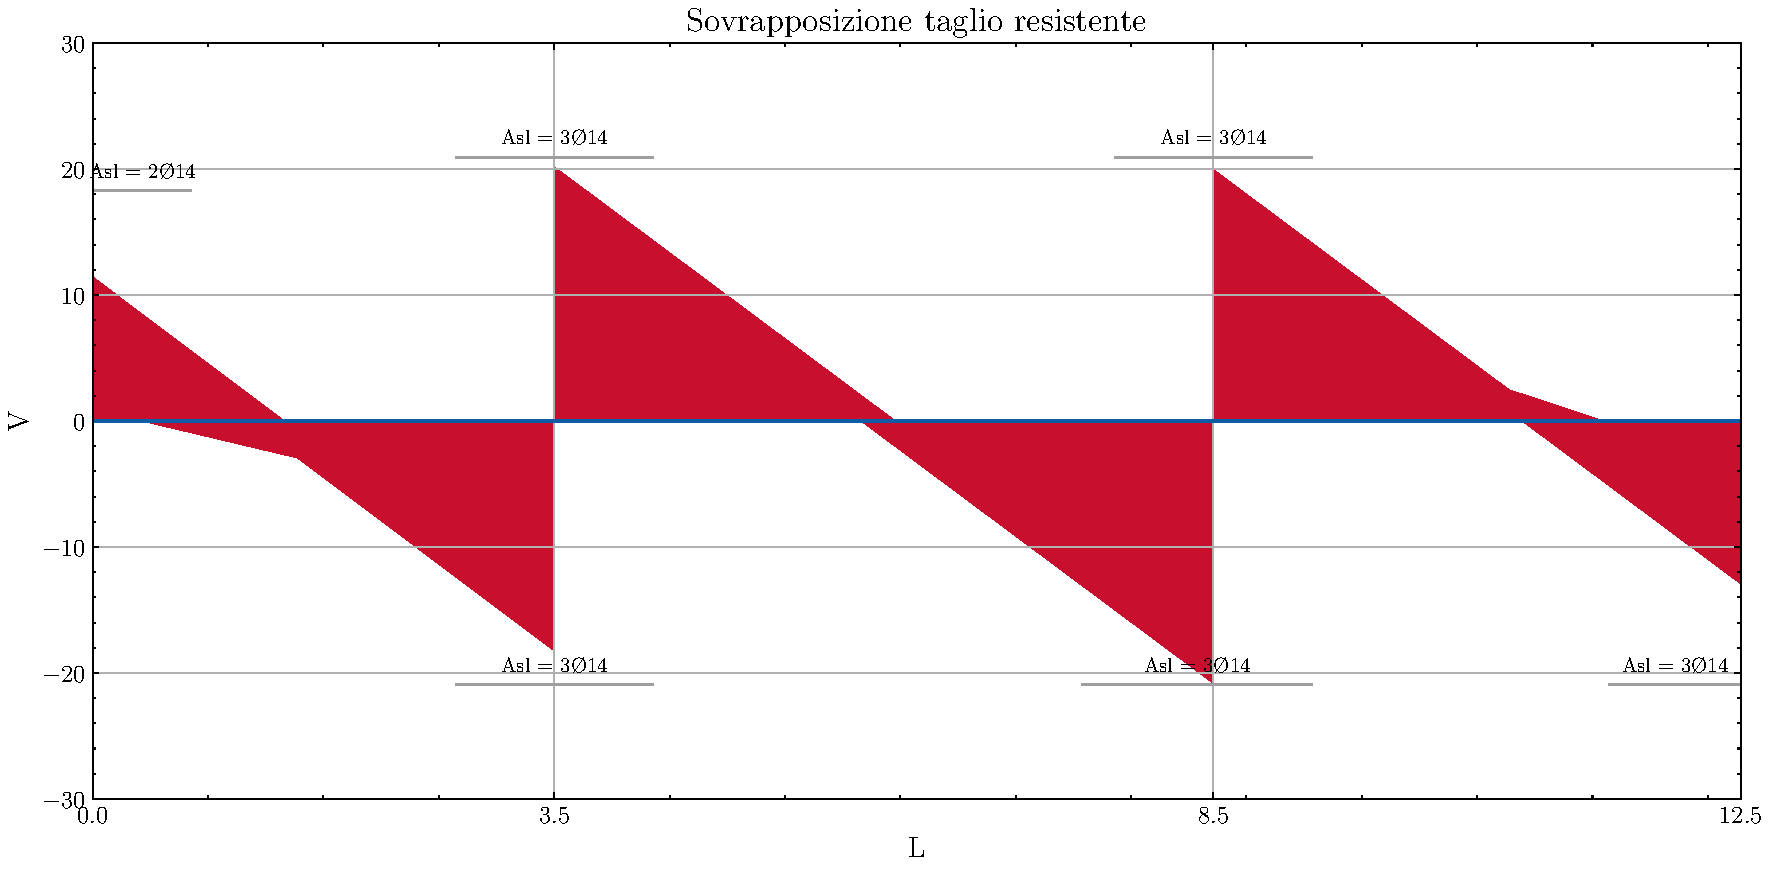
\includegraphics[width=\textwidth]{IMG/ULS_V_DisposioneArmature_solaio.pdf}
    \caption{Sovrapposizione taglio resistente e taglio agente}
    \label{fig:ULS_M_ULS_V_DisposioneArmature_solaio}
\end{figure}